% =============================================================================
%  Thesis Presentation: A Unified GNN + RL + LLM Framework for Fraud Detection
%  Compile with: pdflatex Presentation.tex   (run twice for outline/refs)
%
%  Theme notes:
%    * Primary theme: `metropolis` (modern, clean, professional).
%      Requires the `beamertheme-metropolis` package.
%    * If metropolis is not installed, swap `\usetheme{metropolis}` for
%      `\usetheme{Madrid}` or `\usetheme{CambridgeUS}` (both built-in).
% =============================================================================

\documentclass[aspectratio=169,10pt]{beamer}

% --- theme ---------------------------------------------------------------
\usetheme{metropolis}
% Fallback if metropolis is unavailable (comment the line above, uncomment one below):
% \usetheme{Madrid}
% \usetheme{CambridgeUS}

% --- packages ------------------------------------------------------------
\usepackage[utf8]{inputenc}
\usepackage[T1]{fontenc}
\usepackage{amsmath,amssymb,amsfonts}
\usepackage{booktabs}
\usepackage{array}
\usepackage{multirow}
\usepackage{xcolor}
\usepackage{graphicx}
\usepackage{tikz}
\usetikzlibrary{shapes,arrows.meta,positioning,fit,backgrounds,calc}

% --- colours (metropolis-compatible palette) -----------------------------
\definecolor{accent}{HTML}{EB811B}     % metropolis orange
\definecolor{positive}{HTML}{2CA02C}   % green
\definecolor{negative}{HTML}{D62728}   % red
\definecolor{neutral}{HTML}{1F77B4}    % blue
\definecolor{lightgray}{HTML}{F0F0F0}

% --- metadata ------------------------------------------------------------
\title{A Unified GNN + RL + LLM Framework \\ for Graph-Based Fraud Detection}
\subtitle{Extending CARE-GNN with Learned Policy and LLM Reasoning}
\author{Fady Hassanein}
\institute{Master's Thesis}
\date{\today}

% --- presentation --------------------------------------------------------
\begin{document}

% =========================================================================
%  TITLE SLIDE
% =========================================================================
\begin{frame}
    \titlepage
\end{frame}

% =========================================================================
%  OUTLINE
% =========================================================================
\begin{frame}{Outline}
    \tableofcontents
\end{frame}

% =========================================================================
%  1.  MOTIVATION
% =========================================================================
\section{Motivation and Problem}

\begin{frame}{Why Graph-Based Fraud Detection?}
    \textbf{Online fraud is expensive and networked.}
    \begin{itemize}
        \item Fake reviews on Amazon/Yelp distort consumer decisions and merchant revenue.
        \item Fraudsters don't act alone---they form \emph{rings}: coordinated users,
              burst-posted reviews, shared IP ranges, identical text templates.
        \item A single-user classifier misses the \emph{network evidence}.
    \end{itemize}
    \vspace{0.5em}
    \textbf{Graph Neural Networks (GNNs)} exploit this structure by propagating
    information across user/review relationships.
\end{frame}

\begin{frame}{The Camouflage Problem}
    Fraudsters actively evade detection:
    \begin{itemize}
        \item[\textcolor{negative}{$\bullet$}]\textbf{Feature camouflage:} mimic legitimate users
              (normal ratings, plausible review length, boilerplate sentiment).
        \item[\textcolor{negative}{$\bullet$}]\textbf{Relation camouflage:} form ties to benign users
              to dilute the suspicious signal in neighbourhood aggregation.
    \end{itemize}
    \vspace{0.5em}
    A naive GNN aggregates \emph{all} neighbours and inherits both attacks.
    \vspace{0.5em}
    \begin{alertblock}{Research Question}
        Can we build a GNN that filters neighbours adaptively, incorporates
        semantic reasoning, and remains interpretable---\emph{without} sacrificing
        scalability or reproducibility?
    \end{alertblock}
\end{frame}

% =========================================================================
%  2.  LITERATURE REVIEW AT A GLANCE
% =========================================================================
\section{Literature Review}

\begin{frame}{Progression of Fraud-Detection Methods}
    \begin{center}
    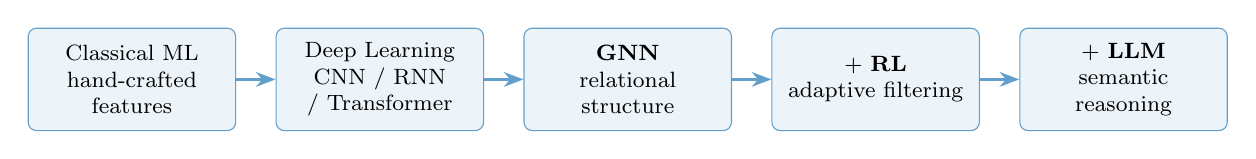
\begin{tikzpicture}[
        node distance=1.2cm and 0.5cm,
        stage/.style={rectangle, rounded corners=3pt, draw=neutral!70, fill=neutral!8,
                      text width=2.4cm, align=center, minimum height=1.3cm, font=\footnotesize},
        arrow/.style={-{Stealth[length=2.5mm]}, thick, neutral!70}
    ]
        \node[stage] (c) {Classical ML \\ hand-crafted features};
        \node[stage, right=of c] (d) {Deep Learning \\ CNN / RNN / Transformer};
        \node[stage, right=of d] (g) {\textbf{GNN} \\ relational structure};
        \node[stage, right=of g] (r) {+ \textbf{RL} \\ adaptive filtering};
        \node[stage, right=of r] (l) {+ \textbf{LLM} \\ semantic reasoning};

        \draw[arrow] (c) -- (d);
        \draw[arrow] (d) -- (g);
        \draw[arrow] (g) -- (r);
        \draw[arrow] (r) -- (l);
    \end{tikzpicture}
    \end{center}
    \vspace{0.3em}
    \begin{itemize}\small
        \item \textbf{Classical ML}: effective baselines, but ignore relational topology.
        \item \textbf{Deep learning}: stronger features, but nodes treated independently.
        \item \textbf{GNNs}: end-to-end relational learning (GCN, GraphSAGE, GAT, \ldots).
        \item \textbf{GNN + RL}: CARE-GNN (Dou~et~al.\ 2020) adds a bandit-based neighbour filter.
        \item \textbf{GNN + LLM}: FLAG (Yang~et~al.\ 2025) uses text for neighbour sampling.
    \end{itemize}
\end{frame}

\begin{frame}{Research Gap}
    \textbf{No existing work unifies all three components:}
    \vspace{0.5em}
    \begin{itemize}
        \item Existing RL + GNN frameworks (CARE-GNN, RioGNN) use simple
              \emph{heuristic bandits} with no semantic state.
        \item Existing LLM + GNN work (FLAG) augments features or sampling but
              does \emph{not} use a learned RL policy for dynamic weighting.
    \end{itemize}
    \vspace{0.8em}
    \begin{exampleblock}{This Thesis}
        A unified \textbf{GNN + RL + LLM} framework that combines:
        \begin{itemize}
            \item A multi-relation \textbf{GNN backbone} (CARE-GNN).
            \item A learned \textbf{actor--critic RL policy} for per-node filtering.
            \item \textbf{LLM-derived signals} injected into both the policy state
                  and the node features.
        \end{itemize}
    \end{exampleblock}
\end{frame}

% =========================================================================
%  3.  FRAMEWORK OVERVIEW
% =========================================================================
\section{The Unified Framework}

\begin{frame}{Three-Pillar Architecture}
    \begin{center}
    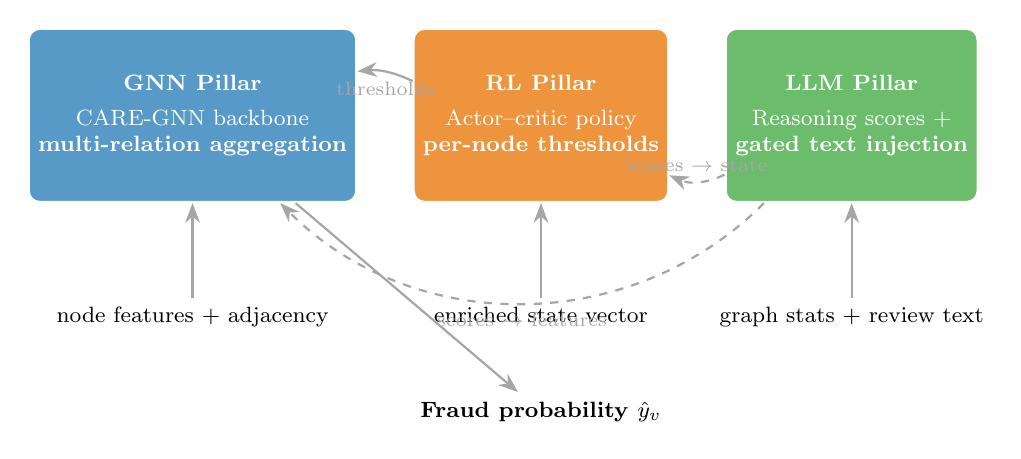
\begin{tikzpicture}[
        node distance=0.6cm and 0.7cm,
        pillar/.style={rectangle, rounded corners=4pt, draw=white, line width=0.8pt,
                       minimum width=3.2cm, minimum height=2.2cm, align=center,
                       font=\footnotesize\bfseries, text=white},
        gnn/.style={pillar, fill=neutral!75},
        rl/.style={pillar, fill=accent!85},
        llm/.style={pillar, fill=positive!70},
        flow/.style={-{Stealth[length=2.5mm]}, thick, gray!70}
    ]
        % three pillars
        \node[gnn] (g) {GNN Pillar \\[3pt]
            \footnotesize\mdseries
            CARE-GNN backbone \\ multi-relation aggregation};
        \node[rl, right=of g] (r) {RL Pillar \\[3pt]
            \footnotesize\mdseries
            Actor--critic policy \\ per-node thresholds};
        \node[llm, right=of r] (l) {LLM Pillar \\[3pt]
            \footnotesize\mdseries
            Reasoning scores + \\ gated text injection};

        % inputs
        \node[below=1.2cm of g, font=\footnotesize] (gin) {node features + adjacency};
        \node[below=1.2cm of r, font=\footnotesize] (rin) {enriched state vector};
        \node[below=1.2cm of l, font=\footnotesize] (lin) {graph stats + review text};

        \draw[flow] (gin) -- (g);
        \draw[flow] (rin) -- (r);
        \draw[flow] (lin) -- (l);

        % integration arrows between pillars
        \draw[flow, dashed] (l) to[bend left=25] node[above, font=\scriptsize]{scores $\to$ state} (r);
        \draw[flow, dashed] (l) to[bend left=45] node[below, font=\scriptsize]{scores $\to$ features} (g);
        \draw[flow] (r) to[bend right=15] node[below, font=\scriptsize]{thresholds} (g);

        % output
        \node[below=2.4cm of r, font=\footnotesize\bfseries] (out) {Fraud probability $\hat{y}_v$};
        \draw[flow] (g) -- (out);
    \end{tikzpicture}
    \end{center}
    \vspace{0.2em}
    \footnotesize
    Each pillar is \emph{additive}: LLM signals flow into the RL state \emph{and}
    the GNN features; the RL policy produces thresholds the GNN consumes.
\end{frame}

\begin{frame}{Design Principle: Additive, Attributable Pillars}
    \textbf{Every design choice preserves two interoperability constraints:}
    \begin{enumerate}
        \item Each pillar enters the framework at a \emph{well-defined interface}
              (feature space, policy state, or threshold variable).
        \item Enabling or disabling a pillar leaves the other two's code unchanged.
    \end{enumerate}
    \vspace{0.5em}
    \textbf{Why this matters:}
    \begin{itemize}
        \item The three-pillar ablation in Chapter~4 measures each pillar's
              contribution cleanly.
        \item Reproducibility: pillar toggles correspond to single command-line flags.
        \item Future extensions (new LLMs, different policies) slot in without
              refactoring the backbone.
    \end{itemize}
\end{frame}

% =========================================================================
%  4.  DATASETS
% =========================================================================
\section{Datasets}

\begin{frame}{Benchmark Datasets}
    \begin{center}
    \begin{tabular}{@{}lcc@{}}
        \toprule
        \textbf{Property} & \textbf{Amazon} & \textbf{YelpChi} \\
        \midrule
        Nodes (total / labelled) & 11{,}944 / 8{,}639 & 45{,}954 / 45{,}954 \\
        Features                 & 25 raw            & 32 pre-normalised \\
        Fraud rate (labelled)    & 9.50\%            & 14.53\% \\
        Relations                & UPU, USU, UVU     & RUR, RTR, RSR \\
        Max $|r|$ feature        & 0.654 (feat.\ 19) & 0.235 (feat.\ 5) \\
        Strongest relation       & UVU (18.3\% / 3.0\%) & \textbf{RUR (92.5\% / 0.4\%)} \\
        Review text available?   & No                & \textbf{Yes} \\
        \bottomrule
    \end{tabular}
    \end{center}
    \vspace{0.5em}
    \begin{itemize}\footnotesize
        \item \textbf{Amazon}: strong per-node features, modest structural homophily.
              Features already solve most of the problem.
        \item \textbf{YelpChi}: weak per-node features. RUR's near-perfect label
              homophily is the main signal---but generic relations (RTR, RSR) are noisy.
        \item Both statistics recomputed from the release used in this thesis.
    \end{itemize}
\end{frame}

% =========================================================================
%  5.  METHODOLOGY — PILLAR 1 (GNN)
% =========================================================================
\section{Methodology: The GNN Pillar}

\begin{frame}{GNN Backbone: CARE-GNN}
    \textbf{Single-layer, multi-relation GNN with label-aware filtering.}
    \vspace{0.4em}
    \begin{enumerate}
        \item \textbf{Label predictor} $S(v) = \mathrm{MLP}(x_v) \in \mathbb{R}^2$
              produces per-node class logits.
        \item \textbf{Pairwise distance}
              $D(v, v') = |S(v)[0] - S(v')[0]|$ ranks neighbours by label agreement.
        \item \textbf{Filter}: retain the top-$p_r$ fraction by distance in each
              relation $r$.
        \item \textbf{Intra-relation aggregation}: mean of retained neighbours.
        \item \textbf{Inter-relation aggregation}:
              $h_v = \mathrm{ReLU}\!\left( W h_v + \sum_r p_r W h_{\mathcal{N}(v)}^{(r)} \right)$.
    \end{enumerate}
    \vspace{0.4em}
    \textbf{What we replace in the unified framework:}
    \begin{itemize}
        \item Step~1's linear predictor $\to$ two-layer MLP with dropout (CAPN).
        \item Step~3's $p_r$ updated by $\epsilon$-greedy bandit $\to$ learned actor--critic policy.
        \item Steps~2, 4, 5 are \emph{retained unchanged}.
    \end{itemize}
\end{frame}

% =========================================================================
%  6.  METHODOLOGY — PILLAR 2 (RL)
% =========================================================================
\section{Methodology: The RL Pillar}

\begin{frame}{From Heuristic Bandit to CAPN}
    \textbf{Inherited bandit (CARE-GNN):}
    \begin{itemize}
        \item Action: $p_r \leftarrow p_r \pm 0.02$, updated \emph{once per epoch}.
        \item Reward: $\pm 1$ based on sign of change in positive-node distance.
        \item Terminal condition: freezes once reward plateaus.
    \end{itemize}
    \vspace{0.3em}
    \begin{alertblock}{Five Limitations}
        Global (not per-node) thresholds $\bullet$ binary reward
        $\bullet$ slow fixed-step updates $\bullet$ linear label predictor
        $\bullet$ \textbf{no hook for external signals (LLM)}.
    \end{alertblock}
    \vspace{0.3em}
    \textbf{CAPN (ours):} Camouflage-Aware Policy Network---a learned neural policy
    that addresses all five limitations through:
    \begin{itemize}
        \item An enhanced two-layer MLP label predictor with confidence output.
        \item A rich state vector (features + distance + overlap + feature variance + LLM scores).
        \item A Beta-distribution policy network that outputs per-node thresholds.
        \item A shaped, continuous reward combining distance + accuracy + stability.
    \end{itemize}
\end{frame}

\begin{frame}{Actor--Critic Policy Optimisation}
    \textbf{Problem:} vanilla REINFORCE has high gradient variance---batch-level
    rewards bounce, the policy oscillates, YelpChi training diverges.
    \vspace{0.5em}
    \textbf{Solution:} single-step actor--critic with a learned value baseline.
    \begin{align*}
        \hat{A}_t &= R_t - \operatorname{sg}\!\bigl[V_\phi(\mathbf{s}_t)\bigr]\\
        \mathcal{L}_{\text{policy}} &= -\hat{A}_t \sum_r \log \pi_\theta(\tau_r\mid\mathbf{s}_t^r)
            - \lambda_H\, H[\pi_\theta]\\
        \mathcal{L}_{\text{critic}} &= \bigl(V_\phi(\mathbf{s}_t) - R_t\bigr)^2
    \end{align*}
    \vspace{0.3em}
    \textbf{Training schedule:}
    \begin{itemize}\footnotesize
        \item Epochs 0--5 (\emph{GNN warmup}): $\lambda_\pi = 0$, only supervised loss runs.
        \item Epochs 5--10 (\emph{policy ramp}): linearly anneal $\lambda_\pi$ from 0 to 0.3.
        \item Epochs 10--31: full policy training at $\lambda_\pi = 0.3$.
    \end{itemize}
\end{frame}

% =========================================================================
%  7.  METHODOLOGY — PILLAR 3 (LLM)
% =========================================================================
\section{Methodology: The LLM Pillar}

\begin{frame}{LLM as Reasoning Engine, Not Text Encoder}
    \textbf{Why not sentence-transformer embeddings?}
    \begin{itemize}
        \item Study A6 tried this on Amazon: 384-dim MiniLM embeddings projected into
              the policy state. Result: \textbf{$-0.19$pp AUC (failed).}
        \item Root cause: lossy round-trip converts precise numerics (degree = 23) to
              text and back, destroying the signal that was already in the state.
    \end{itemize}
    \vspace{0.5em}
    \textbf{Our approach:} use \textbf{Claude Haiku~4.5} as a reasoning engine.
    Two complementary signal streams:
    \begin{center}
    \begin{tabular}{@{}p{3.4cm}p{3cm}p{3.6cm}@{}}
        \toprule
        & \textbf{Part 1 (both datasets)} & \textbf{Part 2 (YelpChi only)} \\
        \midrule
        Input to LLM   & 26 graph statistics per node & raw review text \\
        Output         & 6 structural risk scores     & 6 text risk scores \\
        Entry point    & CAPN state vector            & node features (via gate) \\
        \bottomrule
    \end{tabular}
    \end{center}
    \vspace{0.3em}
    \footnotesize
    All LLM scores are \emph{precomputed once} and loaded as tensors---no API
    calls inside the training loop. Reproducible at zero ongoing cost.
\end{frame}

\begin{frame}{Part 1: Structural Reasoning Scores}
    \textbf{26 graph statistics per node} $\rightarrow$ Claude Haiku 4.5 $\rightarrow$
    \textbf{6 risk scores}:
    \vspace{0.3em}
    \begin{itemize}\footnotesize
        \item \texttt{structural\_anomaly} --- unusual connectivity pattern
        \item \texttt{relation\_consistency} --- uniform behaviour across relations
        \item \texttt{neighborhood\_risk} --- suspicious neighbours (training-label stats)
        \item \texttt{feature\_anomaly} --- statistical feature outliers
        \item \texttt{coordination\_signal} --- likelihood of coordinated activity
        \item \texttt{isolation\_score} --- peripheral vs deeply embedded
    \end{itemize}
    \vspace{0.4em}
    \textbf{Why LLM over linear formula?}
    The LLM can reason about \emph{interactions}: ``high ego-density \emph{combined with}
    high label disagreement \emph{in a single relation}'' signals a fraud ring---
    a linear formula misses the conjunction.
    \vspace{0.4em}
    \textbf{Integration:} 6-score vector $\rightarrow$ linear projector $\rightarrow$
    16-dim $\mathbf{e}_v$ concatenated into CAPN state. \\
    State dimension grows $D{+}5 \to D{+}21$.
\end{frame}

\begin{frame}{Part 2: Text-Risk Scoring and Gated Injection}
    \textbf{YelpChi only} (Amazon ships no review text).
    Six \emph{fraud-specific} text scores per review:
    \vspace{0.2em}
    \begin{itemize}\footnotesize
        \item \texttt{generic\_language}, \texttt{sentiment\_mismatch}, \texttt{promotional\_tone}
        \item \texttt{copy\_paste\_signal}, \texttt{detail\_authenticity}, \texttt{behavioral\_anomaly}
    \end{itemize}
    \vspace{0.4em}
    \textbf{How not to inject:} Study A8 concatenated scores to features $\rightarrow$
    $-0.59$pp AUC (widened weight matrix absorbs noise).
    \vspace{0.2em}
    \textbf{TextFeatureGate (ours):} residual with learnable per-dim sigmoid gate,
    \[
        x'_v \;=\; x_v \;+\; \sigma(g) \odot \bigl( W_{\text{text}}\, t_v \bigr),
        \qquad g \text{ initialised to } -2,\ \sigma(-2)\!\approx\!0.12.
    \]
    \vspace{-0.2em}
    \textbf{Why it works:}
    \begin{itemize}\footnotesize
        \item Preserves original feature dimension ($\mathbb{R}^{32}\!\to\!\mathbb{R}^{32}$).
        \item Gate starts near zero: network behaves almost like CARE-GNN initially.
        \item Training can \emph{unlearn} harmful dimensions by pushing $g$ back to $-\infty$.
    \end{itemize}
\end{frame}

% =========================================================================
%  8.  UNIFIED TRAINING OBJECTIVE
% =========================================================================
\section{Unified Training}

\begin{frame}{Joint Training Objective}
    \textbf{Single end-to-end loss combining all four signals:}
    \[
        \mathcal{L} =
        \underbrace{\mathcal{L}_{\text{GNN}} + \lambda_1\, \mathcal{L}_{\text{sim}}}_{\text{backbone}}
        \;+\; \lambda_\pi(t)\, \mathcal{L}_{\text{policy}}
        \;+\; \lambda_c\, \mathcal{L}_{\text{critic}}
    \]
    \vspace{0.4em}
    \textbf{Dual-optimiser setup:}
    \begin{itemize}
        \item Backbone optimiser: Adam, LR $10^{-2}$, clip max-norm 1.0.
        \item Policy/critic optimiser: Adam, policy LR $3\!\cdot\!10^{-3}$,
              critic LR $10^{-3}$, clip max-norm 5.0.
    \end{itemize}
    \vspace{0.4em}
    \textbf{Why two optimisers?} The actor--critic and the backbone converge on
    different timescales---a single learning rate destabilises training.
\end{frame}

% =========================================================================
%  9.  RESULTS
% =========================================================================
\section{Results}

\begin{frame}{Experimental Protocol}
    \begin{itemize}
        \item \textbf{Splits:} stratified 25\% / 15\% / 60\% train / val / test.
        \item \textbf{Epochs:} 31; best-validation-AUC checkpoint.
        \item \textbf{Seeds:} three seeds $\{72, 73, 74\}$ on YelpChi (mean $\pm$ std);
              single seed $=72$ for Amazon ablations.
        \item \textbf{Metrics:} AUC-ROC and Average Precision (primary); F1-macro,
              Precision, Recall (secondary).
    \end{itemize}
    \vspace{0.6em}
    \textbf{Thesis claim tested:}
    \begin{itemize}
        \item[] \emph{The three-pillar combination (GNN + RL + LLM) significantly
              outperforms CARE-GNN on YelpChi.}
    \end{itemize}
\end{frame}

\begin{frame}{Headline Result (YelpChi)}
    \vspace{0.8em}
    \begin{center}
    \Large
    \textcolor{accent}{\textbf{AUC} \quad $\mathbf{0.7856 \pm 0.0022}$} \\[0.4em]
    \textcolor{accent}{\textbf{AP} \quad\;\; $\mathbf{0.4108 \pm 0.0052}$} \\[0.4em]
    \textcolor{accent}{\textbf{F1-macro} \quad $\mathbf{0.6099 \pm 0.0565}$}
    \end{center}
    \vspace{0.8em}
    \begin{center}\normalsize
    \textbf{+1.99\,pp} AUC over our own same-split CARE-GNN reproduction\\[0.3em]
    Welch's $t$-test: $p < 0.001$ across three seeds.
    \end{center}
\end{frame}

\begin{frame}{Main Table: Three-Pillar Ablation on YelpChi}
    \begin{center}\small
    \begin{tabular}{@{}lccc@{}}
        \toprule
        \textbf{Configuration} & \textbf{AUC} & \textbf{AP} & \textbf{F1-macro} \\
        \midrule
        Row 1: GNN only (CARE-GNN)    & $0.7657 \pm 0.0007$ & $0.3766 \pm 0.0038$ & $0.5948 \pm 0.0263$ \\
        Row 2: GNN + RL               & $0.7681 \pm 0.0005$ & $0.3837 \pm 0.0007$ & $0.5968 \pm 0.0109$ \\
        Row 3: GNN + LLM              & $0.7797 \pm 0.0038$ & $0.3983 \pm 0.0146$ & $0.5927 \pm 0.0578$ \\
        \textbf{Row 4: GNN + RL + LLM} & $\mathbf{0.7856 \pm 0.0022}$ & $\mathbf{0.4108 \pm 0.0052}$ & $\mathbf{0.6099 \pm 0.0565}$ \\
        \bottomrule
    \end{tabular}
    \end{center}
    \vspace{0.5em}
    \textbf{Component contributions (mean AUC):}
    \begin{itemize}\small
        \item \textcolor{positive}{\textbf{+0.24\,pp}} \, Row 1 $\to$ Row 2: RL pillar alone.
        \item \textcolor{positive}{\textbf{+1.40\,pp}} \, Row 1 $\to$ Row 3: LLM pillar alone (dominant).
        \item \textcolor{positive}{\textbf{+0.59\,pp}} \, Row 3 $\to$ Row 4: RL on top of LLM.
    \end{itemize}
    \vspace{0.3em}
    Worst seed of Row 4 ($0.7828$) already beats best seed of Row 1 ($0.7663$) by $+1.65$\,pp.
\end{frame}

\begin{frame}{Statistical Significance}
    Two-sided Welch's $t$-test (three seeds):
    \vspace{0.4em}
    \begin{center}\small
    \begin{tabular}{@{}lccc@{}}
        \toprule
        \textbf{Comparison} & $\Delta\bar{x}$ \textbf{(AUC)} & $t$ & $p$ \\
        \midrule
        Row 4 vs Row 1 (Full vs CARE-GNN)   & $+1.99$\,pp & $\approx 12.4$ & \textcolor{positive}{\textbf{$< 0.001$}} \\
        Row 4 vs Row 2 (Full vs RL only)    & $+1.75$\,pp & $\approx 11.7$ & \textcolor{positive}{\textbf{$< 0.001$}} \\
        Row 4 vs Row 3 (Full vs LLM only)   & $+0.59$\,pp & $\approx 2.7$  & $\approx 0.05$ \\
        \bottomrule
    \end{tabular}
    \end{center}
    \vspace{0.6em}
    \begin{itemize}\small
        \item The full framework is significantly better than CARE-GNN \emph{and}
              than the RL-only variant.
        \item RL-on-top-of-LLM is at the border of conventional significance---would
              be strengthened by expanding the seed pool.
    \end{itemize}
\end{frame}

\begin{frame}{Comparison with the CARE-GNN Paper}
    \begin{center}\small
    \begin{tabular}{@{}lcc@{}}
        \toprule
        \textbf{Model} & \textbf{AUC} & \textbf{Recall} \\
        \midrule
        GCN\textsuperscript{*}                        & 0.5247 & 0.5081 \\
        GAT\textsuperscript{*}                        & 0.5624 & 0.5452 \\
        GraphSAGE\textsuperscript{*}                  & 0.5400 & 0.5286 \\
        GraphConsis\textsuperscript{*}                & 0.6207 & 0.6208 \\
        CARE-GNN\textsuperscript{*}                   & 0.7570 & 0.7192 \\
        \midrule
        Our Row 1 (CARE-GNN reproduction)             & $0.7657 \pm 0.0007$ & $0.6987$ \\
        Our Row 2 (GNN + RL)                          & $0.7681 \pm 0.0005$ & $0.6967$ \\
        Our Row 3 (GNN + LLM)                         & $0.7797 \pm 0.0038$ & $0.6774$ \\
        \textbf{Our Row 4 (GNN + RL + LLM)}           & $\mathbf{0.7856 \pm 0.0022}$ & $0.6923$ \\
        \bottomrule
    \end{tabular}\\[0.2em]
    \footnotesize \textsuperscript{*} Paper-reported values, Dou et al.\ (2020) Table 3, 40\% training data.
    \end{center}
    \vspace{0.5em}
    \footnotesize
    Starred values are literature context at a \emph{different} (40\%) training
    fraction, so no cross-protocol delta is computed against them. The three-pillar
    gain is the \textbf{+1.99\,pp} over our own same-split Row~1 reproduction.
    Recall is slightly lower, consistent with the AUC--Recall trade-off of a
    better-ranking classifier at a fixed decision threshold.
\end{frame}

\begin{frame}{Amazon Component Ablations (A1--A9) Takeaways}
    \begin{itemize}\footnotesize
        \item \textbf{A1 (CAPN vs bandit).} CAPN \textcolor{positive}{$+0.47$\,pp} AUC
              over CARE-GNN; Label AUC \textcolor{positive}{$+5.20$\,pp}.
        \item \textbf{A2 (label predictor).} MLP predictor \emph{alone} hurts GNN AUC
              ($-0.77$\,pp); needs the policy network to realise the gain.
        \item \textbf{A3 (reward shaping).} Any continuous reward beats the binary one;
              the specific decomposition barely matters.
        \item \textbf{A4 (LLM priors).} Best single configuration; $+0.81$\,pp Precision.
        \item \textbf{A5 (sensitivity).} CAPN is robust: AUC varies by $0.0004$ across
              a 50$\times$ range of $\lambda_\pi$.
        \item \textbf{A6 (v1 sentence-transformer).} \textcolor{negative}{FAILED} ($-0.19$\,pp).
              Lossy text round-trip destroyed signal.
        \item \textbf{A7 (v2 reasoning scores).} Reasoning-only: \textcolor{positive}{$+0.05$\,pp AUC,
              $+0.27$\,pp AP}.
        \item \textbf{A8 (feature-level concat).} \textcolor{negative}{FAILED} ($-0.59$\,pp);
              \emph{motivates the gated residual used on YelpChi}.
        \item \textbf{A9 (combined).} No negative interactions---prerequisite for the YelpChi result.
    \end{itemize}
\end{frame}

% =========================================================================
%  10.  CONCLUSION
% =========================================================================
\section{Conclusion}

\begin{frame}{Contributions}
    \begin{enumerate}
        \item A \textbf{unified GNN + RL + LLM framework} for fraud detection,
              architected around a three-pillar, additive design.
        \item \textbf{CAPN}: an actor--critic replacement for CARE-GNN's heuristic
              bandit with per-node thresholds, shaped reward, and LLM-enriched state.
        \item \textbf{Structural LLM reasoning scores} (Part 1): six fraud-specific
              risk scores from Claude Haiku 4.5 over 26 per-node graph statistics.
        \item \textbf{TextFeatureGate} (Part 2): gated residual injection of text-risk
              scores that preserves feature dimension and is \emph{reversible}.
        \item \textbf{Empirical validation}: $+1.99$\,pp AUC on YelpChi with
              $p < 0.001$; nine Amazon ablations attribute each design decision.
    \end{enumerate}
\end{frame}

\begin{frame}{Limitations and Future Work}
    \textbf{Limitations.}
    \begin{itemize}
        \item Three seeds on YelpChi gives tight CIs but limited power for
              border-line effects (Row 3 vs Row 4).
        \item RL pillar tested only on this benchmark family; no ``in the wild''
              evaluation with concept drift.
        \item LLM reasoning prompts are not tuned---the template is frozen.
    \end{itemize}
    \vspace{0.4em}
    \textbf{Future work.}
    \begin{itemize}
        \item Scale to five seeds and additional benchmarks (T-Finance, DGraph-Fin).
        \item End-to-end LLM prompt optimisation (e.g.\ DSPy, reward-model tuning).
        \item Temporal fraud detection: extend CAPN state with time-aware features.
        \item Compare against newer fraud-GNN baselines (GAGA, BWGNN, FLAG).
    \end{itemize}
\end{frame}

% =========================================================================
%  THANK YOU
% =========================================================================
\begin{frame}[standout]
    Thank you \\[0.5em]
    \normalsize Questions?
\end{frame}

\appendix

% =========================================================================
%  APPENDIX (optional backup slides)
% =========================================================================
\begin{frame}{Backup: Dataset Relational Statistics}
    \begin{center}\footnotesize
    \begin{tabular}{@{}lrrrr@{}}
        \toprule
        \textbf{Relation} & $|E|$ (undir.) & Avg.\ Deg. & \% Fraud Nbrs (fraud) & \% Fraud Nbrs (benign) \\
        \midrule
        \multicolumn{5}{c}{\textit{Amazon}} \\
        \midrule
        UPU & 175{,}608     & 29.4  & 10.0 & 4.8 \\
        USU & 3{,}566{,}479 & 597.2 & 10.3 & 3.6 \\
        UVU & 1{,}036{,}737 & 173.6 & 18.3 & 3.0 \\
        \midrule
        \multicolumn{5}{c}{\textit{YelpChi}} \\
        \midrule
        RUR & 49{,}315     & 2.15   & \textbf{92.5} & 0.4  \\
        RTR & 573{,}616    & 24.96  & 18.0 & 14.0 \\
        RSR & 3{,}402{,}743 & 148.09 & 20.5 & 13.5 \\
        \bottomrule
    \end{tabular}
    \end{center}
    \vspace{0.3em}
    \footnotesize
    All statistics recomputed from the adjacency-list release used in this thesis.
    RUR's near-perfect label homophily (92.5\% fraud nbrs for fraud nodes) is the
    dominant structural signal on YelpChi.
\end{frame}

\begin{frame}{Backup: Unified Training Hyperparameters}
    \begin{center}\footnotesize
    \begin{tabular}{@{}lc@{}}
        \toprule
        \textbf{Hyperparameter} & \textbf{Value} \\
        \midrule
        Policy weight target $\lambda_\pi^{\star}$       & 0.3 \\
        Similarity loss weight $\lambda_1$                & 2 \\
        Critic loss weight $\lambda_c$                    & 0.1 \\
        Entropy coefficient $\lambda_H$                   & 0.01 \\
        GNN warmup epochs $E_{\text{warm}}$               & 5 \\
        Policy ramp epochs $E_{\text{ramp}}$              & 5 \\
        Backbone LR                                       & $1 \times 10^{-2}$ \\
        Policy LR                                         & $3 \times 10^{-3}$ \\
        Critic LR                                         & $1 \times 10^{-3}$ \\
        Backbone gradient clip (max-norm)                 & 1.0 \\
        Policy / critic gradient clip (max-norm)          & 5.0 \\
        Optimiser                                         & Adam (two instances) \\
        Batch size (YelpChi / Amazon)                     & 1{,}024 / 256 \\
        Epochs                                            & 31 \\
        TextFeatureGate init $g$                          & $-2$ (sigmoid $\approx 0.12$) \\
        \bottomrule
    \end{tabular}
    \end{center}
\end{frame}

\end{document}
